\subsection{Context Viewpoint}
    
    % \subsubsection{Concerns}
    %     As stated in section \ref{desc:context}, the primary concern is that the experience of actors should not inhibit their ability to use the product.
    %     The product targets one user, so each use case will only have one actor.
        
    \subsubsection{Elements}
        \paragraph{Switch subsystem}
           The user shall be able to switch between looping subsystem and modulation subsystem.
          
                \begin{figure}[!ht]
                    \centering
                    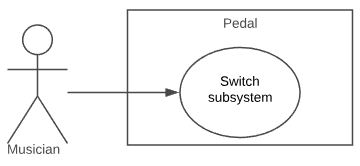
\includegraphics[width=.5\textwidth]{diagrams/use_cases/uc-switch.JPG}
                    \caption{Switch subsystem use case}
                    \label{fig:uc-switch}
                \end{figure}
            
        \begin{table}[!ht]
            \centering
            \begin{tabular}{ l l  }
                Use Case & Switch subsystem  \\
                \hline \\
                Use Case Number & 1 \\ \\
                Summary & Musician can switch between the looping subsystem and the modulation subsystem. \\ \\
                Actor & Musician \\ \\
                Trigger & Hardware input: button or switch \\ \\
                
                Pre-Conditions & The pedal must be in either the looping subsystem or the modulation subsystem  \\ \\
                Post-Conditions & If the pedal was initially in the modulation system, it must be in the looping system. \\ 
                & If the pedal was initially in the looping system, it must be in the modulation system. \\ \\
                Assumptions & The pedal is powered on \\ \\
            \end{tabular}
            % \\
            % \caption{Use case: Switch subsystem}
            % \label{tab:uc-switch}
        \end{table}
    
        \clearpage
        \paragraph{Start recording audio} 
        The user shall be able to record audio to playback later.
                    \begin{figure}[!ht]
                \centering
                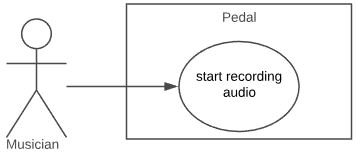
\includegraphics[width=.5\textwidth]{diagrams/use_cases/uc-record-start.JPG}
                \caption{Start recording audio use case}
                \label{fig:uc-record-start }
            \end{figure}
        \begin{table}[!ht]
            \centering
            \begin{tabular}{ l  l  }
                Use Case & Start recording audio  \\ \hline \\
                Use Case Number & 2 \\ \\
                Summary & Musician can start recording audio. \\ \\
                Actor & Musician \\ \\
                Trigger & Hardware input: pedal toggle \\ \\
                Pre-Conditions & The pedal must be in the looping subsystem. \\
                & The looping subsystem must not already be recording. \\ \\
                Post-Conditions & The looping subsystem will be recording incoming audio. \\ \\
                Assumptions & The user has audio input plugged in.\\
            \end{tabular}
            % \\
            % \caption{Use case: Start recording audio}
            % \label{tab:uc-record-start}
        \end{table}
        
 
        \paragraph{Stop recording audio} 
            The user shall be able to record audio to playback later.
            \begin{figure}[!ht]
                \centering
                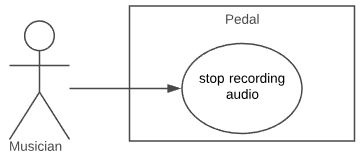
\includegraphics[width=.5\textwidth]{diagrams/use_cases/uc-record-stop.JPG}
                \caption{Stop recording audio use case}
                \label{fig:uc-record-stop }
            \end{figure}
            
            \clearpage
            
            \begin{table}[!ht]
                \centering
                \begin{tabular}{ l  l }
                    Use Case & Stop recording audio  \\
                    \hline \\
                    Use Case Number & 3 \\ \\
                    Summary & Musician can stop recording audio. \\ \\
                    Actor & Musician \\ \\
                    Trigger & Hardware input: pedal toggle \\ \\
                    Pre-Conditions & The pedal must be in the looping subsystem. \\
                    & The looping subsystem must be recording audio. \\ \\
                    Post-Conditions & The looping subsystem will cache the recorded audio. \\ \\
                    Assumptions & The user has audio input plugged in.\\ 
                \end{tabular}
                % \\
                % \caption{Use case: Stop recording audio}
                % \label{tab:uc-record-stop}
            \end{table}
 
      
        \paragraph{Start audio playback} 
            The user shall be able to playback recorded audio.
            \begin{figure}[!ht]
                \centering
                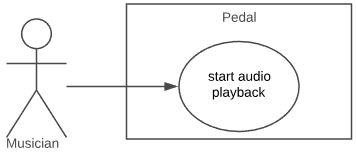
\includegraphics[width=.5\textwidth]{diagrams/use_cases/uc-play-start.JPG}
                \caption{Start audio playback use case}
                \label{fig:uc-play-start}
            \end{figure}
            \begin{table}[!ht]
                \centering
                \begin{tabular}{l l}
                    Use Case & Start audio playback \\ 
                    \hline \\
                    Use Case Number & 4 \\ \\
                    Summary & Musician can start playing back audio. \\ \\
                    Actor & Musician \\ \\
                    Trigger & Hardware input: pedal toggle \\ \\
                    Pre-Conditions & The pedal must be in the looping subsystem. \\
                    & The looping subsystem must have audio cached. \\ \\
                    Post-Conditions & The looping subsystem will begin audio playback. \\ \\
                    Assumptions & None.\\ 
                \end{tabular}
                % \\
                % \caption{Use case: Start audio playback}
                % \label{tab:uc-play-start}
            \end{table}
    
           \clearpage
            \paragraph{Stop audio playback} 
            The user shall be able to stop the playback recorded audio.
            \begin{figure}[!ht]
                \centering
                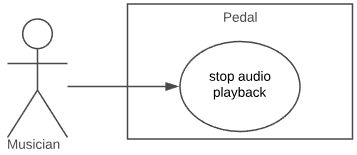
\includegraphics[width=.5\textwidth]{diagrams/use_cases/uc-play-stop.JPG}
                \caption{Stop audio playback use case}
                \label{fig:uc-play-stop}
            \end{figure}
            \begin{table}[!ht]
                \centering
                \begin{tabular}{l l}
                    Use Case & Stop audio playback \\ 
                    \hline \\ 
                    Use Case Number & 5 \\ \\
                    Summary & Musician can stop audio playback. \\ \\
                    Actor & Musician \\ \\
                    Trigger & Hardware input: pedal toggle \\ \\
                    Pre-Conditions & The pedal must be in the looping subsystem. \\
                    & The looping subsystem must have audio cached. \\
                    & The looping subsystem must be currently playing audio back \\ \\
                    Post-Conditions & The looping subsystem will stop audio playback. \\ \\
                    Assumptions & None.\\
                \end{tabular}
                % \\
                % \caption{Use case: Stop audio playback}
                % \label{tab:uc-play-stop}
            \end{table}
            
            \paragraph{Select effect} 
            The user shall be able to select an effect.
            \begin{figure}[!ht]
                \centering
                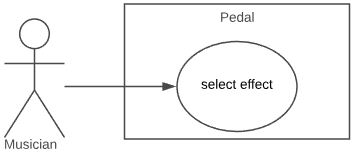
\includegraphics[width=.5\textwidth]{diagrams/use_cases/uc-select-effect.JPG}
                \caption{Select effect use case}
                \label{fig:uc-select-effect}
            \end{figure}
            \clearpage
            \begin{table}[!ht]
                \centering
                \begin{tabular}{l l}
                    Use Case & Select effect \\
                    \hline \\
                    Use Case Number & 6 \\ \\
                    Summary & Musician can select an effect to use on the pedal. \\ \\
                    Actor & Musician \\ \\
                    Trigger & Hardware input: selector \\ \\
                    Pre-Conditions & The pedal must be in the modulation subsystem. \\
                    & The audio effect library must have effects. \\ \\
                    Post-Conditions & The modulation subsystem will load an effect to a cache. \\ \\
                    Assumptions & None.\\ \\
                \end{tabular}
                % \\
                % \caption{Use case: Select effect}
                % \label{tab:uc-select-effect}
            \end{table}            
            
            \paragraph{Start effect} 
            The user shall be able to start using an effect.
            \begin{figure}[!ht]
                \centering
                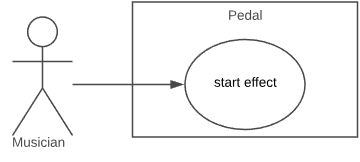
\includegraphics[width=.5\textwidth]{diagrams/use_cases/uc-effect-start.JPG}
                \caption{Start effect use case}
                \label{fig:uc-start-effect}
            \end{figure}
            \begin{table}[!ht]
                \centering
                \begin{tabular}{l l}
                    Use Case & Start effect \\
                    \hline \\
                    Use Case Number & 7 \\ \\
                    Summary & Musician can start using an effect to modulate incoming audio. \\ \\
                    Actor & Musician \\ \\
                    Trigger & Hardware input: pedal toggle \\ \\
                    Pre-Conditions & The pedal must be in the modulation subsystem. \\
                    & The corresponding pedal toggle must have an effect cached. \\ \\
                    Post-Conditions & The modulation subsystem will start modulating incoming audio. \\ \\
                    Assumptions & An incoming audio signal exists.\\ \\
                \end{tabular}
                % \\
                % \caption{Use case: Start effect}
                % \label{tab:uc-start-effect}
            \end{table}     
            
            \paragraph{Stop effect} 
            The user shall be able to stop using an effect.
            \begin{figure}[!ht]
                \centering
                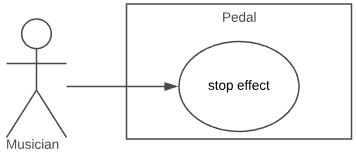
\includegraphics[width=.5\textwidth]{diagrams/use_cases/uc-effect-stop.JPG}
                \caption{Stop effect use case}
                \label{fig:uc-stop-effect}
            \end{figure}
            \begin{table}[!ht]
                \centering
                \begin{tabular}{l l}
                    Use Case & Stop effect \\
                    \hline \\
                    Use Case Number & 8 \\ \\
                    Summary & Musician can stop using an effect to modulate incoming audio. \\ \\
                    Actor & Musician \\ \\
                    Trigger & Hardware input: pedal toggle \\ \\
                    Pre-Conditions & The pedal must be in the modulation subsystem. \\
                    & An effect must be running. \\ \\
                    Post-Conditions & The modulation subsystem will stop modulating incoming audio. \\ \\
                    Assumptions & An incoming audio signal exists.\\ \\
                \end{tabular}
                % \\
                % \caption{Use case: Stop effect}
                % \label{tab:uc-stop-effect}
            \end{table}     